\renewcommand{\figurename}{Diagram}
In this paper we introduce translation mechanism for the fundamental concepts employed by Subversion and Git.
\emph{Translator} is the server-side implementation of this mechanism.
\subsection{Notation}
This specification uses two-layer notation to illustrate translation scenarios. First layer represents 
Subversion history as a sequence of revisions (revision is represented by a set of red circles located in the same row), while second layer represents Git repository history
as a sequence of Git commits (green circles) connected with child-parent relationship (arrows pointing from the child 
commit to the parent one). 
\\\\
Combination of these two layers in a single diagram provides example of a particular translation scenario by
establishing connection between Git repository and Subversion repository histories. Connection is established
by putting Git commits on top of the corresponding parts of Subversion revisions, whenever such correspondence exists.
\\\\
Refer to the following three diagrams for individual layers notation and example of a combined history diagram.
\subsubsection{Subversion history layer}
\begin{center}
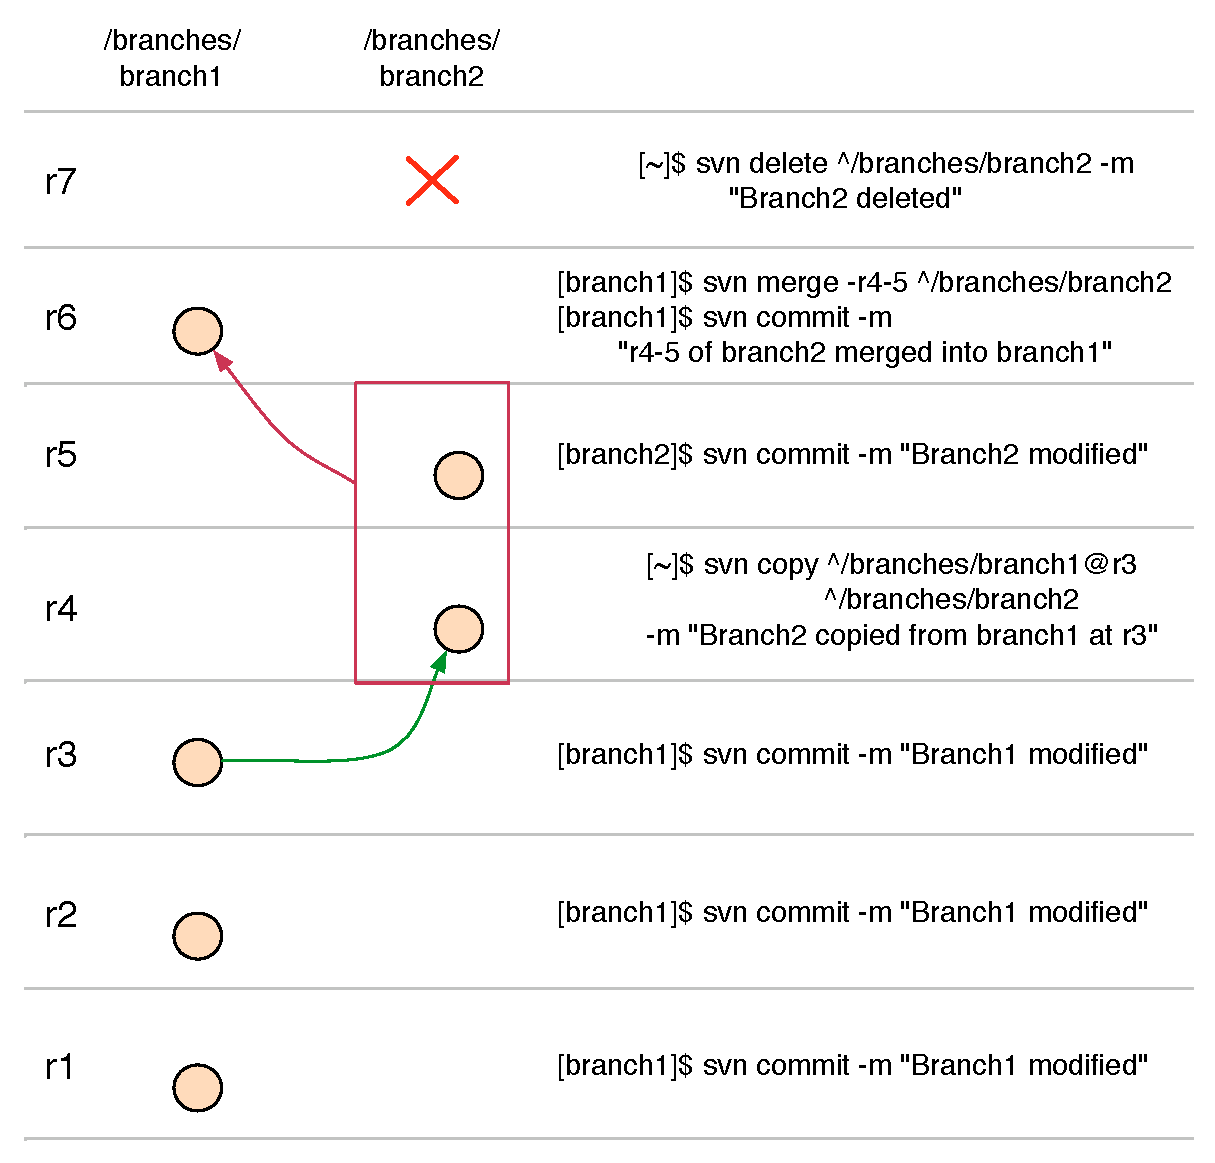
\includegraphics[width=\textwidth]{img/legend/svn_layer.pdf}%
\captionof{figure}{Subversion history layer.}
\label{svn_layer}%
\end{center}
Each row represents single Subversion revision. Each row might contain one or more circles which represent
modifications of the corresponding branches in Subversion repository enclosed in a single revision. A special
case of modification is branch deletion, which is depicted as a red cross instead of circle.\\\\
Copies are shown with green arrows and merge tracking references with the red ones.
\subsubsection{Git history layer}
\begin{center}
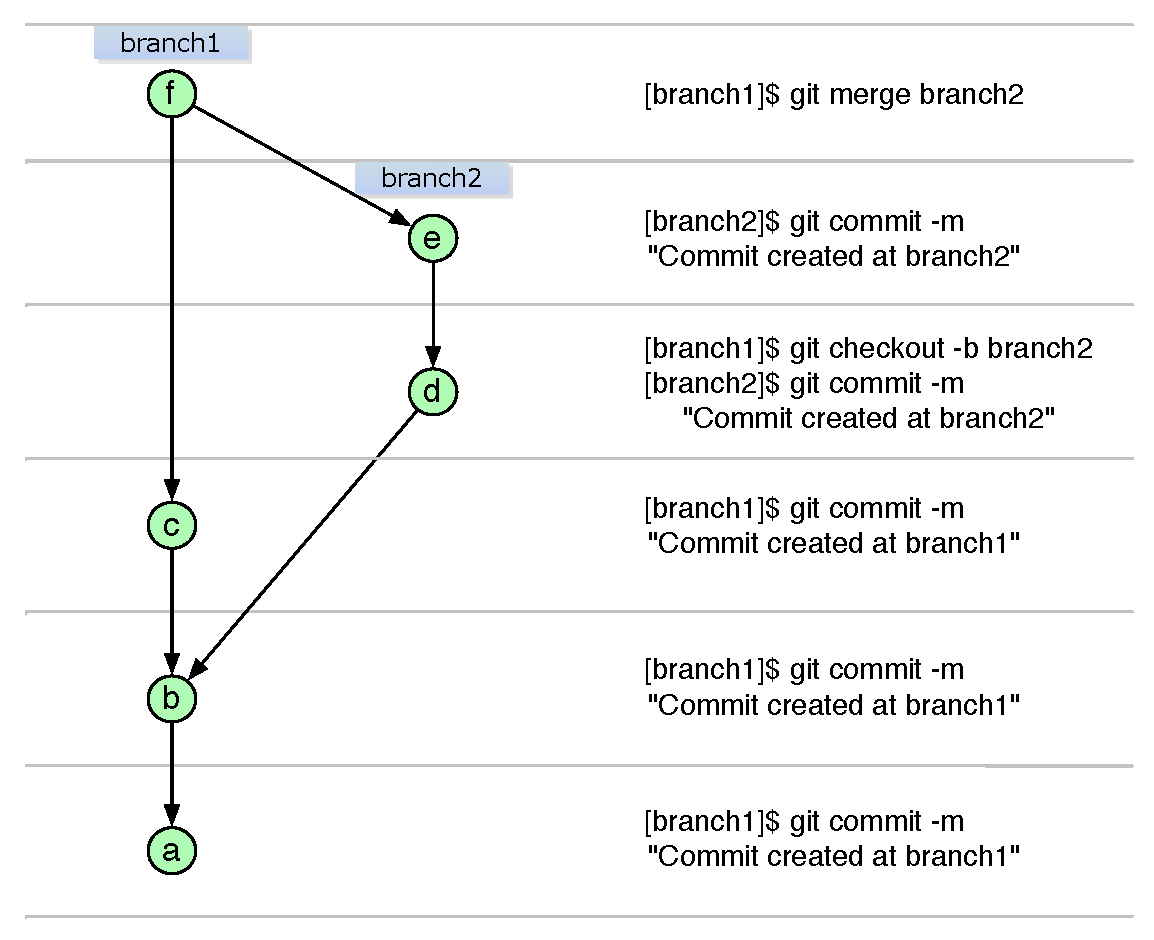
\includegraphics[width=\textwidth]{img/legend/git_layer.pdf}%
\captionof{figure}{Git history layer.}
\label{git_layer}%
\end{center}
When Git commit has more than one parent (e.g. commit \emph{f}), link to the first parent is drawn as a vertical arrow and links to the other 
parents are drawn as an oblique arrow.
\subsubsection{Combined history diagram}
\begin{center}
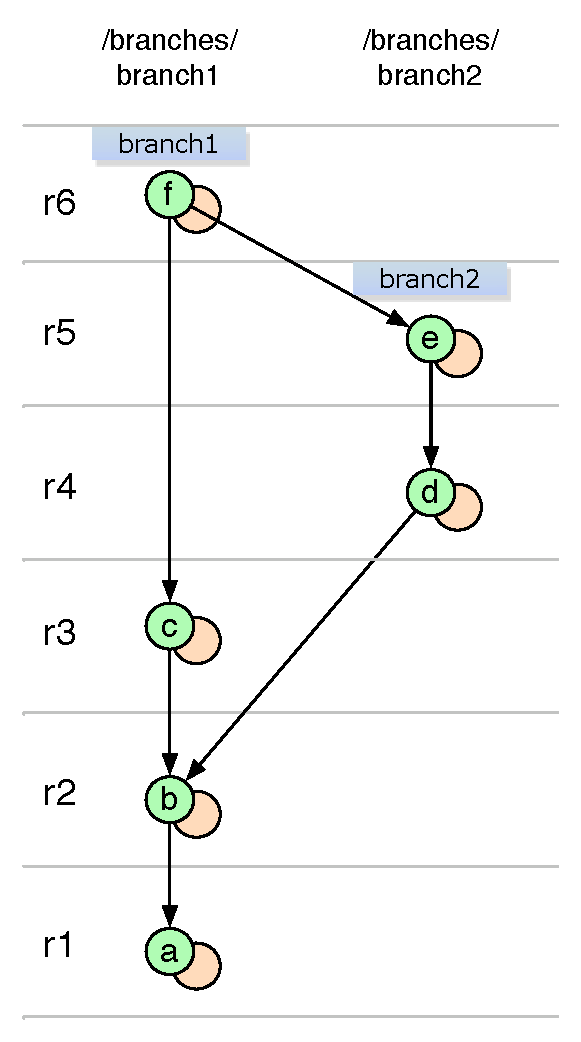
\includegraphics[width=7.0cm]{img/legend/generalized_history.pdf}%
\captionof{figure}{Combined history.}
\label{both_layers}%
\end{center}

Combined history diagram is a result of a two layers combination, where Git commits (green circles) are put on top of the corresponding Subversion revisions (red circles). 
In certain translation scenarios there might be no correspondence between particular Git commit and Subversion revision.